\documentclass[../main/main.tex]{subfiles}
\begin{document}
\chapter{Quantum Optimal Control}
\section{QOC Theory}
Quantum Optimal Control applies OC-solutions to drive the evolution of a quantum system in a fixed time $\tau$. The goal of this process is to obtain, at the end of the time evolution, a final state with the desired properties. A QOC problem is completely defined in terms of the system dynamics, the control objectives, and the control space restrictions \cite{optimal_control_NV_centers}. The evolution of pure states is described by the Schrödinger equation. A generalized equation holds for the evolution of mixed states. The Hamiltonian that describes the system dynamics is decomposed into a constant drift Hamiltonian $\hat{H}_d$ and a time-dependent control Hamiltonian $\hat{H}_c(t) = \sum_i u_i(t) \hat{H}_{i,c}$ in which the control pulses $u_i(t)$ enters as a constant factor input of Hamiltonians $\hat{H}_{i,c}$. The control objectives are defined in terms of a function $J$, the \textit{cost function} or \textit{figure of merit}. The ultimate goal of QOC is to find the control pulses $u_i(t)$ that minimize $J$. The optimal control pulses will be, then, applied in the experiments to get the desired evolution. The cost function evaluates numerically how the evolution controlled by the pulses $u_i(t)$ satisfies the goal of the optimization. For example, at the end of the evolution of a state $\ket{\psi}$ into a state $\ket{\psi(\tau)}$, $J$ evaluates the distance between $\ket{\psi(\tau)}$ and a target state $\ket{\psi_t}$ computing $J=1-\left|\braket{\psi_t|\psi(\tau)} \right|^2$. Similarly, $J$ can evaluate the distance between an evolved gate $U(\tau)$ and a target one $U_t$. The cost function can also encode physical restrictions, e.g., limitations on the power of the control pulses, limitations on the bandwidth, etc. For example, when a control pulse exceeds the restrictions, a penalty term is added to $J$. More direct restrictions on the control pulses can be realized by adding limitations to the pulses, such as hard walls, or by squeezing the control pulses. \par
Numerical algorithms used in QOC can be divided in gradient-based and gradient-free algorithms. On one side, gradient-based algorithms compute at each iteration the derivative of the cost function $J$ with respect to the control pulses $u_i(t)$. The control pulses are then updated following the direction of the functional derivative. The use of small steps in the algorithm guarantees the improvement of $J$. On the other side, gradient-free algorithms allow an improvement of $J$ without calculating its gradient. This feature is particularly important for optimizations in which the evaluation of the gradient of $J$ is expensive or even impossible.
\subsection{CRAB algorithm} \label{sect:CRAB}
The Chopped RAndom Basis (CRAB) gradient-free algorithm uses a truncated randomized basis of functions in order to simplify the minimization of the cost function $J$ \cite{Caneva_2011,optimal_control_NV_centers}. The algorithm recasts the problem of functional minimization to a multi-variable function minimization exploiting the advantages of a randomized basis of functions. In the following we focus on the basis of trigonometric functions. Fixing the number of basis elements $N_{be}$ and the evolution time $\tau$, a possibility to randomize our trigonometrical basis is to choose the $N_{be}$ frequencies according to
\begin{equation} \label{eq:CRAB_random_freq}
    \omega_i = \frac{2 \pi}{\tau} \left( i - r_i \right),
\end{equation}
with $i=1,\dots,N_{be}$ \cite{optimal_control_NV_centers}. The numbers $r_i$ are picked randomly from a flatten distribution in $[0,1]$. Equation~\eqref{eq:CRAB_random_freq} is  the definition used in the optimizations of Sect.~\ref{sect:optimization_superconducting_qubits}, although in principle other definitions of the random frequencies $\omega_i$ can be chosen. The time-dependent control pulse can be thus written as
\begin{equation} \label{eq:CRAB_control_pulse}
    u(t) = \sum_{i=1}^{N_{be}} \left[ A_i \sin(\omega_i t) + B_i \cos(\omega_i t) \right].
\end{equation}
The cost function depends now on the amplitudes $A_i,B_i$ and at every iteration the minimizing algorithm computes $J$ straightforwardly. A direct search method such as Nelder-Mead \cite{nelder_mead_algorithm} updates the amplitudes (i.e. the control pulse) after each iteration. When the updated control pulse fulfils the algorithm stopping criteria, the optimal control pulse is obtained. \par
A more advanced version of the algorithm, the dressed Chopped RAndom Basis algorithm, or dCRAB, repeats the CRAB routine several times \cite{Rach_2015_dCRAB}. At every repetition of the CRAB algorithm, the so-called superiteration, a new set of frequencies is chosen and the optimal pulse is found. The initialization pulse for every superiteration is chosen to be equal to the optimal pulse of the previous superiteration. The final control pulse is given by the sum of the control pulses of all the superiterations. This improved algorithm allows to avoid the local minima of the cost function and needs less optimization parameter for every CRAB routine, i.e., for every superiteration. However, the CRAB algorithm turns out to be sufficient for the optimizations of Sect.~\ref{sect:optimization_superconducting_qubits} and the improvements of the dCRAB algorithm are not further exploited.
\section{Application to superconducting qubits} \label{sect:optimization_superconducting_qubits}
In this section we show how the implementation of one- and two-qubit gates can be improved with QOC using the CRAB algorithm. We postulate the presence of dephasing effects from the external world and we try to find an optimal pulse that can compensate for these undesired effects. The optimization procedure is similar in both cases.\\
At first the Hamiltonian without external noise is defined. With this Hamiltonian we implement the target gate by switching on its drift part $\hat{H}_d$ for a precise amount of time $\tau$. The evolution time $\tau$ is fixed during the optimization. By fixing $\tau$ we simulate the experimental situation in which the detuning source is constant, the pure states evolve according to Schrödinger equation, and the cost function $J$ is computed from the experimental final state $\ket{\psi (\tau)}$. Then, the control pulses are updated following the optimization algorithm. On our side we can simulate numerically the evolution of $\ket{\psi}$ and then the process is equivalent to the experimental one.\\
In the following optimizations the gate cost function $J$ is defined as
\begin{equation} \label{eq:J_definition}
    J =  1-\frac{1}{N_0^2} \left| Tr( U_t^{\dagger} U(\tau) \right|^2 = 1-\frac{1}{N_0^2} \left| \sum_{i=1}^{N_0} \braket{\zeta_i|U_t^{\dagger}|\phi_i(\tau)} \right|^2.
\end{equation}
In Eq.~\eqref{eq:J_definition} $\ket{\zeta_i}$ are the basis states of the Hilbert space $\mathcal{H}$ of dimension $N_0=\dim \mathcal{H}$. The states $\ket{\phi_i(\tau)}=U(\tau) \ket{\zeta_i}$ are obtained by integrating for a time $\tau$ the Schrödinger equation
\begin{equation} \label{eq:Schrodinger_equation}
    i \frac{d}{dt} \ket{\psi(t)} = H(u_1(t),\dots,u_m(t)) \ket{\psi(t)},
\end{equation}
using $\ket{\zeta_i}$ as the initial state. In all the QOC calculations $\hbar=1$ is intended. We highlight the dependence of the Hamiltonian on the time-dependent control pulses $u_i(t)$, $i=1,\dots,m$. The cost function $J$ defined as in Eq.~\eqref{eq:J_definition} can be interpreted as an esteem of the \textit{infidelity} of the gate, since if $U(\tau)$ tends to $U_t$ then $J$ tends to zero. The task of QOC is thus to minimize the gate cost function or, equivalently, the gate infidelity.
\subsection{Optimization of one-qubit NOT gate}
From Sect.~\ref{sect:1Q_gates_implementation} we know that the NOT gate can be obtained by letting the system evolve, according to the Hamiltonian
\begin{equation} \label{eq:unpert_Hamiltonian_NOT}
    \hat{\tilde{H}}_{1Q} = -\frac{1}{2} B_x\, \hat{\sigma}_x,
\end{equation}
for a time $\tau=\pi/B_x$. The parameter $B_x$ is positive and constant. In the following we define all the physical quantities relatively to $B_x$ to get comparable results and to fix the timescales of the optimization. The numerical value of $B_x$ is ultimately set to $1$ and the time of evolution is thus $\tau=\pi$. In Fig.~\ref{fig:ideal_NOT} it is possible to see that the NOT gate behaves as expected if the system is described exactly by the Hamiltonian~\eqref{eq:unpert_Hamiltonian_NOT}. Small bars are still visible in the diagonal elements of Fig.~\ref{fig:ideal_NOT} because of the finite precision of the integration method. We calculate the value of $J$ as in Eq.~\eqref{eq:J_definition} to have an estimate of the implemented gate infidelity. \par
However, in the real implementation of a NOT gate the Hamiltonian that describes the system could be different from what we expect. Additional terms in the Hamiltonian~\eqref{eq:unpert_Hamiltonian_NOT} can arise from external sources that we can not control. For example, we can model the system by considering in the Hamiltonian~\eqref{eq:unpert_Hamiltonian_NOT} an additional $\hat{\sigma}_z$-term, i.e.,
\begin{equation} \label{eq:pert_Hamiltonian_NOT}
    \hat{H}^*_{1Q} = -\frac{1}{2} B_x\, \hat{\sigma}_x + \beta\, \hat{\sigma}_z .
\end{equation}
The magnitude of this additional term is fixed to $\beta = 0.2\, B_x$. In this thesis, the "noise" is defined as an additional term in the Hamiltonian that deviates the time evolution of a system from the expected one. The time evolution described by the noisy Hamiltonian~\eqref{eq:pert_Hamiltonian_NOT} for a time $\tau = \pi/B_x$ leads to the gate represented in Fig.~\ref{fig:noisy_NOT}. \par
\begin{figure}[ht]
    \begin{minipage}[t]{.45\textwidth}
        \centering
        \makebox[\textwidth][c]{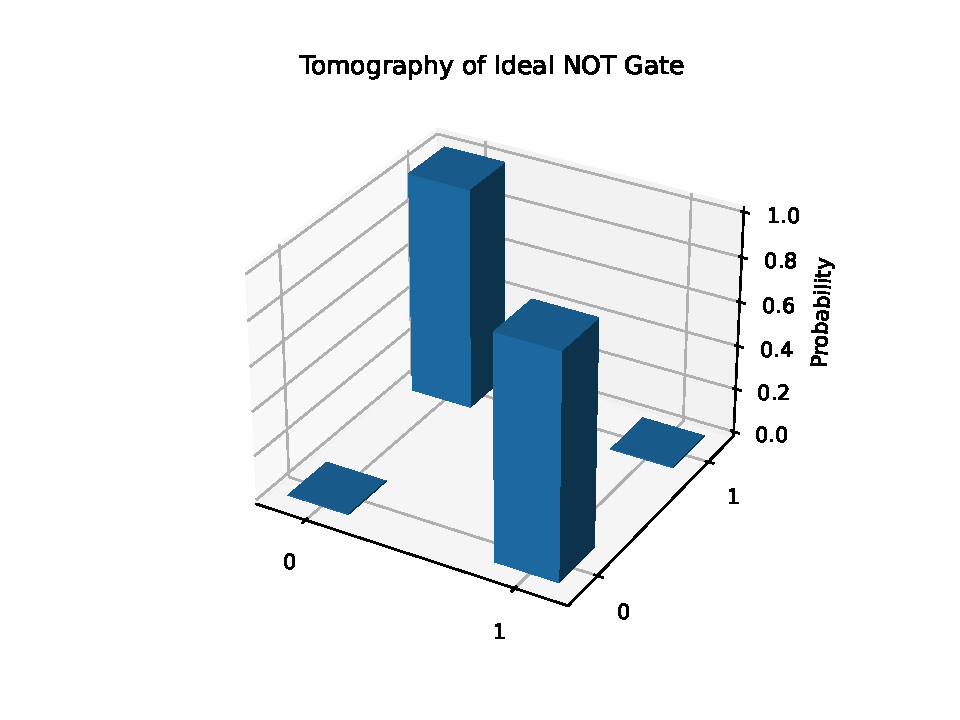
\includegraphics[width=1.3\textwidth]{../images/idealNOT.pdf}}
        \vspace{-1cm}
        \caption{Tomography of the NOT gate in the noiseless approximation. The blue bars represent the probabilities of the corresponding matrix element. The gate infidelity of this implementation is $J=3.8 \cdot 10^{-15}$.}
        \label{fig:ideal_NOT}
    \end{minipage}
    \hfill
    \begin{minipage}[t]{.45\textwidth}
        \centering
        \makebox[\textwidth][c]{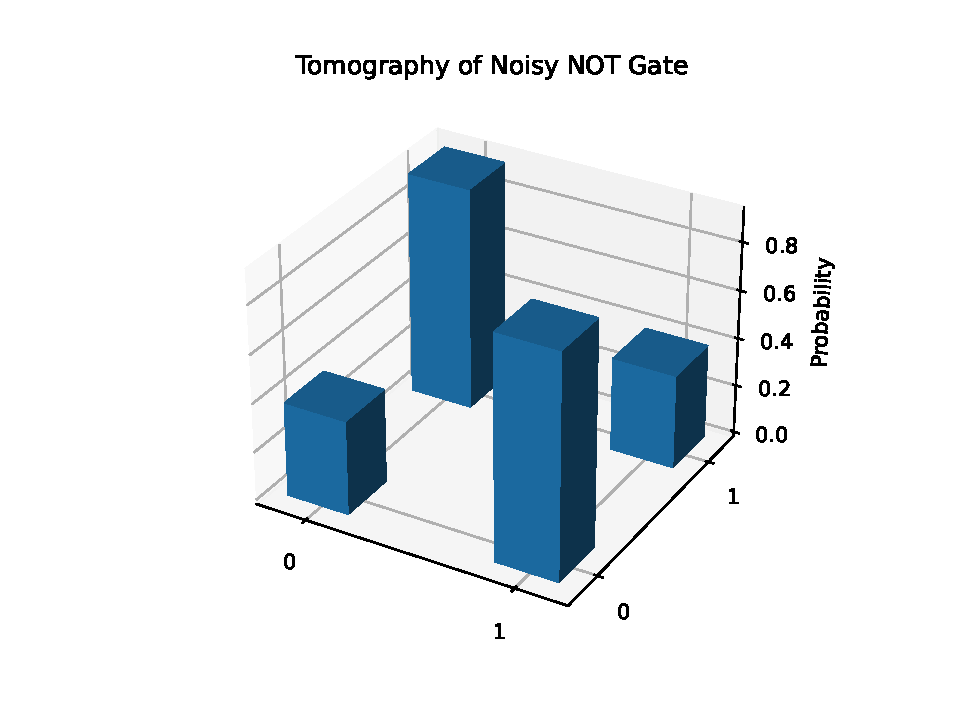
\includegraphics[width=1.3\textwidth]{../images/pertNOT.pdf}}
        \vspace{-1cm}
        \caption{Tomography of the noisy NOT gate. The gate infidelity of this implementation is $J=0.15$.}
        \label{fig:noisy_NOT}
    \end{minipage}
\end{figure}
\vspace{0.5cm}
To improve the implementation of the noisy NOT gate, we add to the Hamiltonian~\eqref{eq:pert_Hamiltonian_NOT} a time-dependent control pulse that generates a rotation around the x-axis. The controlled Hamiltonian is thus
\begin{equation} \label{eq:ctrl_Hamiltonian_NOT}
    \hat{H}_{1Q}(t) = \hat{H}^*_{1Q} + B_x \sum_{i=1}^{N_{be}} \left[ A_i \sin(\omega_i t) + B_i \cos(\omega_i t) \right] \hat{\sigma}_x.
\end{equation}
The definition of the control pulse parameters is reported in Sect.~\ref{sect:CRAB}.\\
In the following one-qubit gate optimization the number of frequencies is set to $N_{be}=3$. The random frequencies are chosen according to Eq.~\eqref{eq:CRAB_random_freq}. The $2 N_{be}$ initialization amplitudes are picked up randomly in the (arbitrary) interval $\left[-\frac{1}{2},\frac{1}{2}\right]$ to set a large initial step to escape local minima.\\
We then employ the Nelder-Mead algorithm \cite{nelder_mead_algorithm} to find the amplitudes $A_i,B_i$ that minimize the cost function $J$. The algorithm starts by transforming the initialization amplitudes into the $2 N_{be}$-dimensional initialization simplex. One vertex of this simplex is the origin, while the others $2 N_{be}$ are generated by translating the origin along each dimension according to the corresponding initial amplitude. Each step of the algorithm computes a new simplex performing reflections, expansions, contractions, and shrinks, using a fixed characteristic parameter for each of these operations. The algorithm computes the value of $J$ for every new vertex found by these operations. The algorithm returns the final amplitudes when one of the convergence criteria is met. We considered three convergence criteria: the maximum number of function evaluations, the maximum number of algorithm iterations, and the difference of both amplitudes and cost function values below a specific tolerance. The first two criteria halt the algorithm if it is requiring excessive time, while the third criterion stops the algorithm when an acceptable precision on the final result is obtained. To be more specific, at every iteration the vertex with the lowest value of $J$ is selected and the differences of its function value and the function values of the other vertices are computed. If all of these differences are below the tolerance value $f_{\text{tol}}$, a similar control is done to the coordinates of all the other vertices with respect to the best vertex. If also all of these differences are below the tolerance value $x_{\text{tol}}$, the algorithm stops successfully and returns the coordinates (i.e., the amplitudes) of the vertex with the lowest value of $J$. In the next optimization we set the maximum number of iterations and the maximum number of function evaluations at $1200$, while we fix $x_{\text{tol}}=10^{-4}$ and $f_{\text{tol}}=10^{-4}$. \par
\begin{figure}[ht]
    \begin{minipage}[t]{.45\textwidth}
        \centering
        \makebox[\textwidth][c]{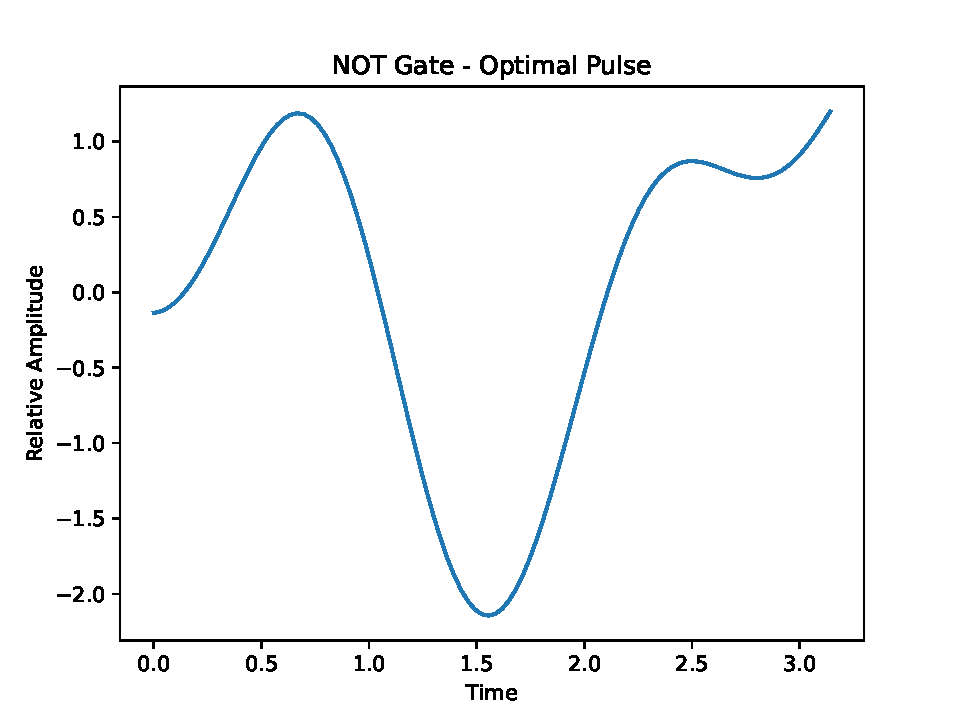
\includegraphics[width=1.3\textwidth]{../images/NOTpulse.pdf}}
        \vspace{-0.5cm}
        \caption{Optimal pulse found by a run of the algorithm. The total time of the pulse is set to $\pi$ and the amplitude on the y-axis is relative to the value of $B_x$.}
        \label{fig:NOT_pulse}
    \end{minipage}
    \hfill
    \begin{minipage}[t]{.45\textwidth}
        \centering
        \makebox[\textwidth][c]{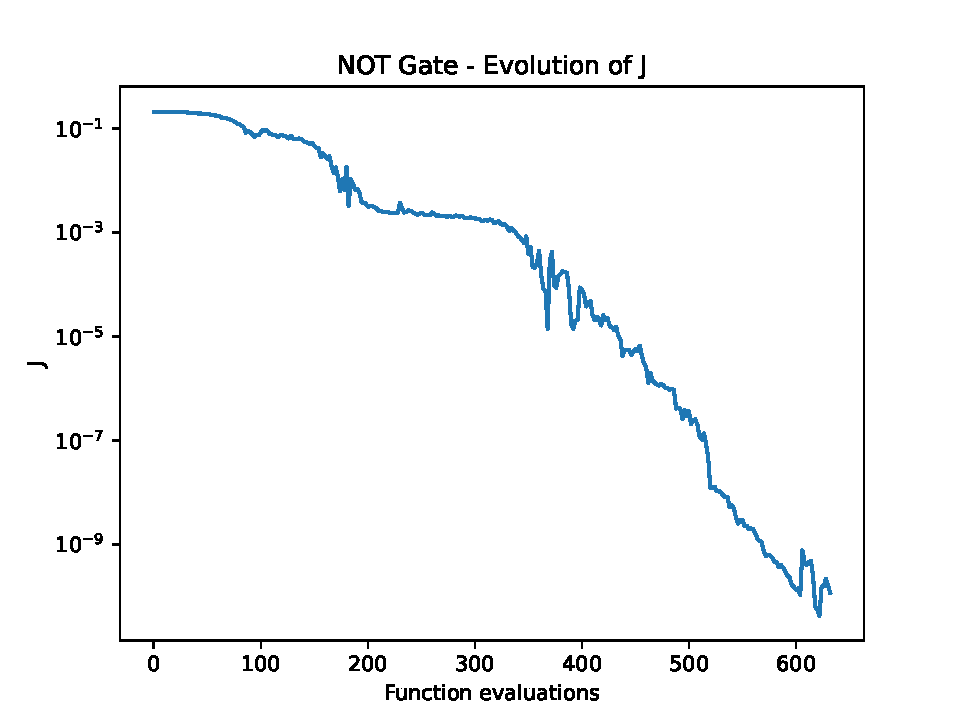
\includegraphics[width=1.3\textwidth]{../images/NOT_evolutionJ.pdf}}
        \vspace{-0.5cm}
        \caption{Evolution of the gate cost function $J$ (in logarithmic scale) over the number of the function evaluations. Only a value of $J$ every 2 evaluations is shown. The final value of the infidelity is \mbox{$J=2.8 \cdot 10^{-11}$}.}
        \label{fig:NOT_evolutionJ}
    \end{minipage}
\end{figure}
\vspace{0.5cm}
Figure~\ref{fig:NOT_pulse} shows a typical pulse obtained by the algorithm, while in Fig.~\ref{fig:NOT_evolutionJ} it is shown in chronological order what are the different function values tested by the algorithm. The spikes indicate vertex guesses that are worse than the vertices already found. The algorithm does not update the simplex in that case, but tries to find a better guess.
\subsection{Optimization of two-qubit CNOT gate}
We know from Eq.~\eqref{eq:CNOT_gate} that the CNOT gate can be obtained by switching on the inter-qubit coupling for a specific timespan and by performing 4 single-qubit operations. We focus only on the optimization of the operations in the square brackets of Eq.~\eqref{eq:CNOT_gate}, while the application of the Hadamard gates to the second qubit is considered as perfect and instantaneous. We have, then, to implement only the two-qubit operation $\exp{\left(i\frac{\pi}{4} \hat{\sigma}_z^1 \hat{\sigma}_z^2 \right)}$ and, for both qubits, the z-rotation $U_z(-\pi/2) \equiv U_z(3\pi/2)$. This implementation is possible considering the Hamiltonian
\begin{equation} \label{eq:unpert_Hamiltonian_CNOT}
    \hat{\tilde{H}}_{2Q} = -\frac{1}{2} B_z^1 \hat{\sigma}_z^1 -\frac{1}{2} B_z^2 \hat{\sigma}_z^2 + E_{CC}\, \hat{\sigma}_z^1 \hat{\sigma}_z^2 .
\end{equation}
Both $B_z^{1,2}$ and $E_{CC}$ are defined relatively to a positive parameter $B_x$ and they can be tuned to realize different operations on the qubits. The implementation of the CNOT gate proceeds in two different steps:
\begin{enumerate}
    \item The two-qubit operation $\exp{\left(i\frac{\pi}{4} \hat{\sigma}_z^1 \hat{\sigma}_z^2 \right)}$ is performed. We fix the inter-qubit coupling to \mbox{$E_{CC}=-0.1\, B_x$} and we set $B_z^1 = B_z^2 = 0$. The evolution time of this step is $\tau_1=\pi/(4\, |E_{CC}|)=\pi/(0.4 \,B_x)$.
    \item The one-qubit operation $U_z(3\pi/2)$ is realized for each qubit. We set $E_{CC}=0$ and we fix $B_z^1 = B_z^2 =-B_x$ instead. The evolution time of this step is $\tau_2 = \pi/(2\,B_x)$.
\end{enumerate}
\begin{figure}[ht]
\vspace{-0.2cm}
    \begin{minipage}[t]{.45\textwidth}
        \centering
        \makebox[\textwidth][c]{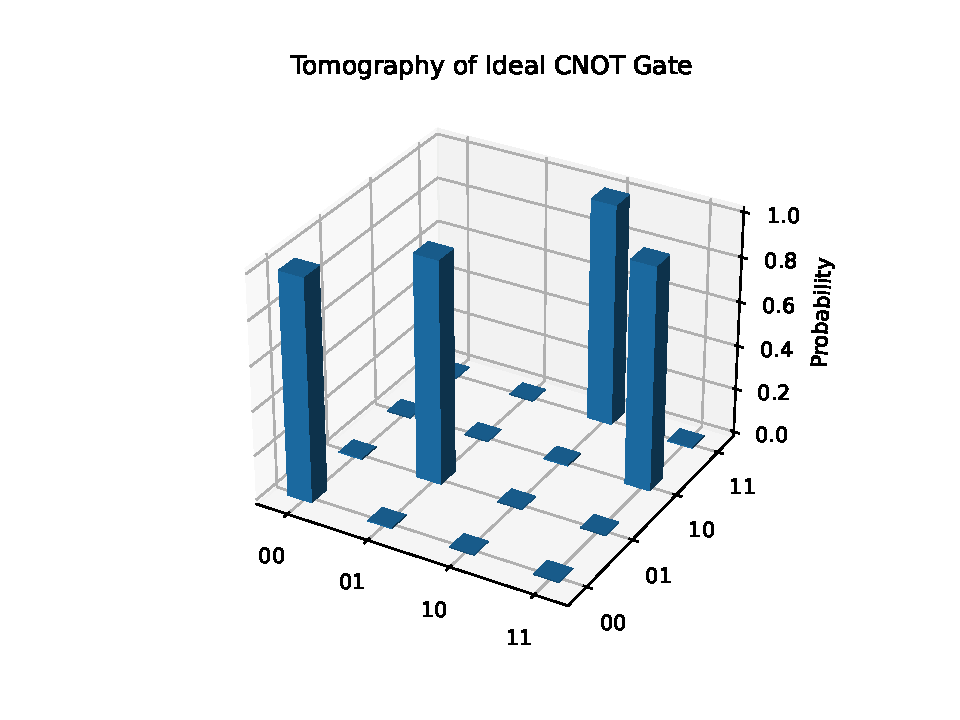
\includegraphics[width=1.3\textwidth]{../images/idealCNOT.pdf}}
        \vspace{-1cm}
        \caption{Tomography of the CNOT gate in the noiseless approximation. The gate infidelity of this implementation is \mbox{$J=2.8 \cdot 10^{-13}$}.}
        \label{fig:ideal_CNOT}
    \end{minipage}
    \hfill
    \begin{minipage}[t]{.45\textwidth}
        \centering
        \makebox[\textwidth][c]{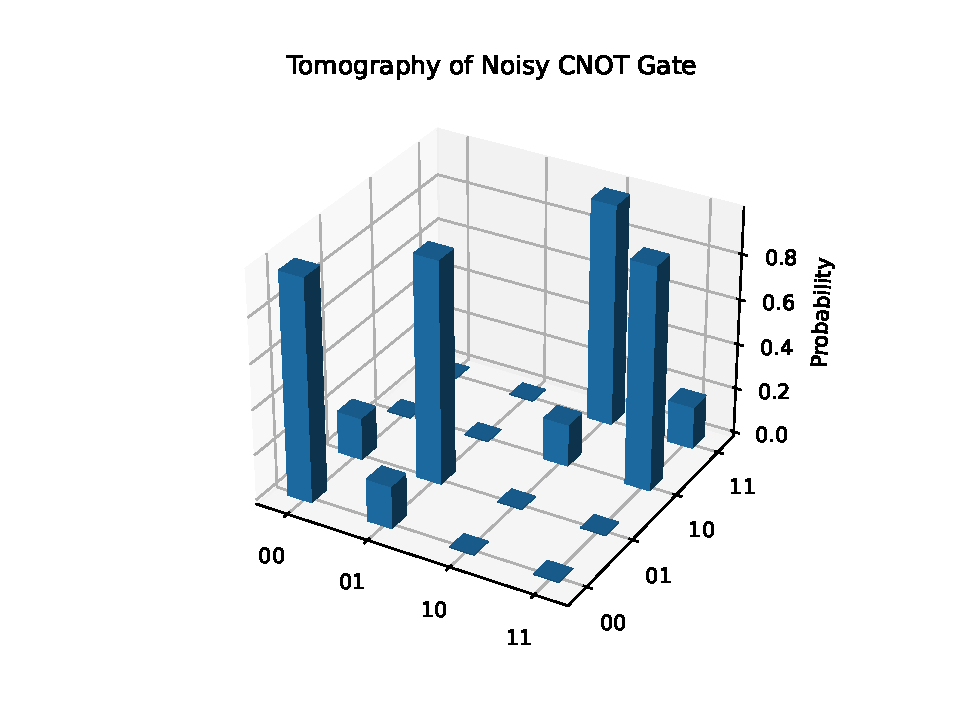
\includegraphics[width=1.3\textwidth]{../images/pertCNOT.pdf}}
        \vspace{-1cm}
        \caption{Tomography of the noisy CNOT gate. The gate infidelity of this implementation is $J=0.069$.}
        \label{fig:noisy_CNOT}
    \end{minipage}
\end{figure}
\vspace{0.5cm}
The value of $B_x$ is set to $1$ as in the one-qubit optimization.\\
In Fig.~\ref{fig:ideal_CNOT} it is shown the aforementioned implementation if the system Hamiltonian is exactly \eqref{eq:unpert_Hamiltonian_CNOT}. This implementation is similar to the target gate to a very good approximation. We can consider, now, two additional terms in the Hamiltonian~\eqref{eq:unpert_Hamiltonian_CNOT} that disturb the expected time evolution, for example
\begin{equation} \label{eq:pert_Hamiltonian_CNOT}
    \hat{H}^*_{2Q} = -\frac{1}{2} B_z^1 \hat{\sigma}_z^1 -\frac{1}{2} B_z^2 \hat{\sigma}_z^2 + E_{CC}\, \hat{\sigma}_z^1 \hat{\sigma}_z^2 + \beta \hat{\sigma}_z^1 + \beta \hat{\sigma}_z^2 .
\end{equation}
These additional terms act on the qubits with the same magnitude $\beta=-0.02\, B_x$ and lead to the gate represented in Fig.~\ref{fig:noisy_CNOT}. These terms are present in both of the two implementation steps described above and they act on the system for a total time of $\tau_1+\tau_2$. The obtained gate behaves differently from the target CNOT gate, so we add controls to the Hamiltonian~\eqref{eq:pert_Hamiltonian_CNOT} to direct its time evolution towards the desired CNOT gate.\\
We optimize the implementation of the two steps described above, while we still consider the application of the Hadamard gate as perfect and instantaneous. In other words, we optimize only the gate
\begin{equation} \label{eq:simple_CNOT_gate}
    U_z^1(-\pi/2)\ U_z^2(-\pi/2)\, \exp{\left(i\frac{\pi}{4} \hat{\sigma}_z^1 \hat{\sigma}_z^2 \right)},
\end{equation}
from which the CNOT gate can be easily obtained. This goal can be achieved by defining a controlled Hamiltonian of the form
\begin{equation} \label{eq:ctrl_Hamiltonian_CNOT}
    \hat{H}_{2Q}(t) = \hat{H}^*_{2Q} + \frac{1}{2} B_x\,  u_1(t)\, \hat{\sigma}_z^1 \hat{\sigma}_z^2 + B_x\, u_2(t)\, \left( \hat{\sigma}_x^1 + \hat{\sigma}_x^2 \right),
\end{equation}
where
\begin{align} \label{eq:pulses_definition_CNOT}
    u_1(t) &= \sum_{i=1}^{N_{be}} \left[ A_i \sin(\omega_i t) + B_i \cos(\omega_i t) \right],
    &
    u_2(t) &= \sum_{i=1}^{N_{be}} \left[ C_i \sin(\omega_i t) + D_i \cos(\omega_i t) \right].
\end{align}
The symmetries of this implementation suggest to use the same $\hat{\sigma}_x$-pulse on the two qubits, reducing the computational cost of the optimization. The random frequencies $\omega_i$ are the same for the $\hat{\sigma}_z^1 \hat{\sigma}_z^2$ and the $\left( \hat{\sigma}_x^1 + \hat{\sigma}_x^2 \right)$ control pulses, but in general different frequencies can be chosen.\\
The two pulses $u_1(t),u_2(t)$ act on the system for the entire time needed by the two-step implementation, i.e., for a total time \mbox{$\tau_1 + \tau_2 = 3\pi/B_x = 3\pi$} if $B_x=1$. We write these two pulses in a truncated trigonometrical basis of $N_{be}=5$ randomized frequencies. The frequencies are chosen according to \eqref{eq:CRAB_random_freq}. The $4 N_{be}$ initialization amplitudes are selected randomly in $\left[ -\frac{1}{2},\frac{1}{2} \right]$. We employ the Nelder-Mead algorithm\footnote{We set the maximum number of iterations and the maximum number of function evaluations at $6000$, we fix $f_{\text{tol}}=10^{-4}$ and we reduce $x_{\text{tol}}$ to $10^{-3}$ to speed up the optimization.} with adaptive parameters \cite{nelder_mead_algorithm,Gao2012}, which is specific for high-dimensional functions minimization. \par
\begin{figure}[ht]
    \begin{minipage}[t]{.45\textwidth}
        \centering
        \makebox[\textwidth][c]{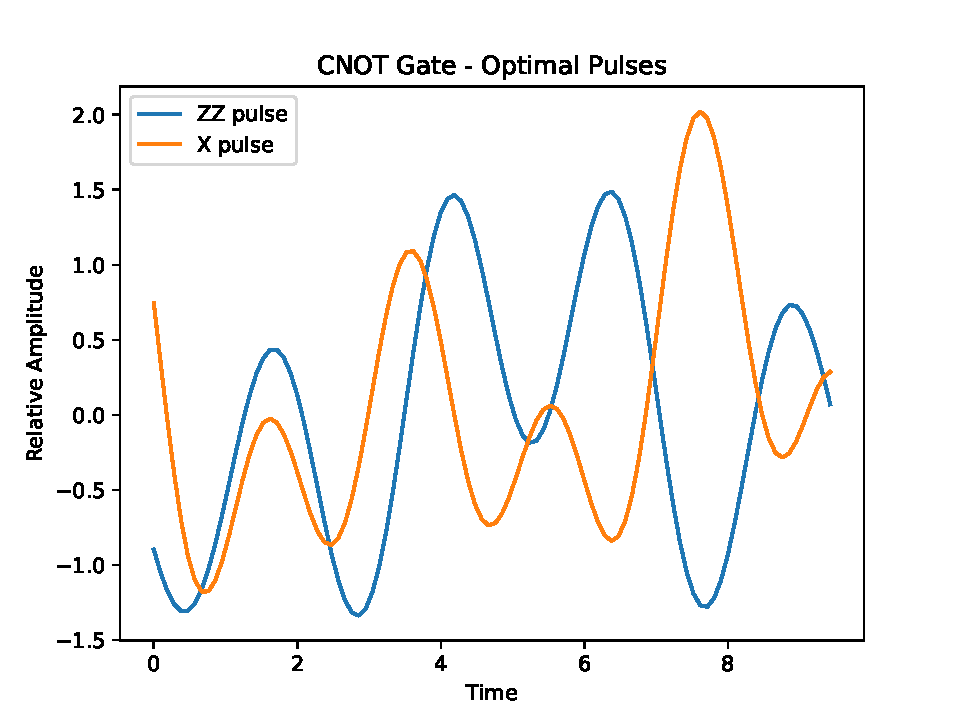
\includegraphics[width=1.3\textwidth]{../images/CNOTpulse.pdf}}
        \vspace{-0.5cm}
        \caption{Optimal pulses found by a run of the algorithm. The total time of the pulses is set to $3\pi$. The amplitudes on the y-axis correspond to $u_1(t)$ for the zz-pulse and to $u_2(t)$ for the x-pulse.}
        \label{fig:CNOT_pulse}
    \end{minipage}
    \hfill
    \begin{minipage}[t]{.45\textwidth}
        \centering
        \makebox[\textwidth][c]{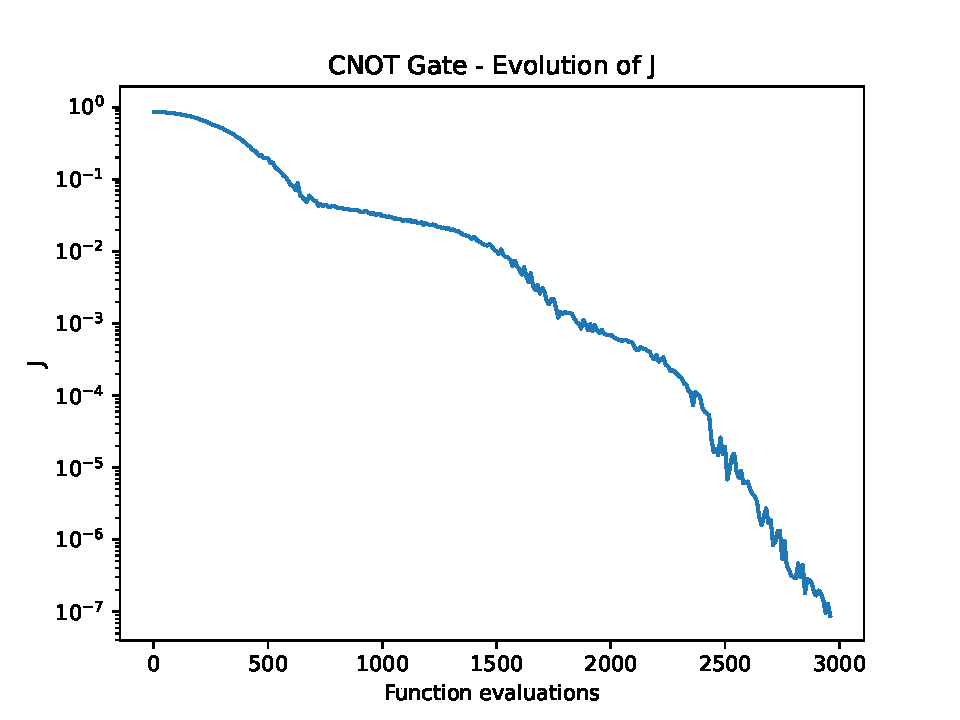
\includegraphics[width=1.3\textwidth]{../images/CNOT_evolutionJ.pdf}}
        \vspace{-0.5cm}
        \caption{Evolution of the gate cost function $J$ (in logarithmic scale) over the number of the function evaluations. Only a value of $J$ every 10 evaluations is shown. The final value of the infidelity is \mbox{$J=8.7 \cdot 10^{-8}$}.}
        \label{fig:CNOT_evolutionJ}
    \end{minipage}
\end{figure}
\vspace{0.5cm}
Figure~\ref{fig:CNOT_pulse} shows the two pulses computed by the optimization algorithm, while the evolution of the value of $J$ over the number of function evaluations is shown in Fig.~\ref{fig:CNOT_evolutionJ}. Here we point out the difference in the function evaluations between the two types of optimization we have performed. The higher number of dimensions of the two-qubit cost function with respect to the one-qubit cost function leads to more expensive computations. Indeed, our two-qubit optimization requires about five times more function evaluations than our single-qubit one. The final value of the gate infidelity is also three orders of magnitude greater in the two-qubit optimization than in one-qubit.\\
Similar difficulties are found experimentally: the setup that implements a two-qubit gate is longer to prepare and needs more time to evolve to the desired one. Thus, if decoherence times are limited, in the software development the number of two-qubit operations performed should be minimized. Nevertheless, two-qubit gates are fundamental building blocks of quantum computation and they can not be excluded from quantum algorithms.
\end{document}